% Slide 1 — Nhắc lại Hypothesis 2

% ============================================================
% HYPOTHESIS 2 — THEORY
% ============================================================

\section{Hypothesis 2 — Verification}

\begin{frame}{Hypothesis 2: Gradient Signal}

\textbf{Hypothesis 2:}

Nếu LM loss thay đổi theo retrieval coefficient $d$, gradient
\[
\frac{\partial L_{\mathrm{LM}}}{\partial d}
\]
có thể cung cấp tín hiệu cục bộ cho retrieval decision.

\vspace{0.3cm}

\textbf{Gradient Interpretation}
\begin{itemize}
    \item $\frac{\partial L_{\mathrm{LM}}}{\partial d}<0$:
    Tăng $d$ có xu hướng giảm LM loss.

    \item $\frac{\partial L_{\mathrm{LM}}}{\partial d}>0$:
    Tăng $d$ có xu hướng tăng LM loss.
\end{itemize}

\vspace{0.2cm}

\textbf{Verification:}
Đo gradient tại 33 decision levels:
\[
d \in \{0/32,1/32,\ldots,32/32\}.
\]

\end{frame}

% Slide 2 — Example

% ============================================================
% HYPOTHESIS 2 — EXAMPLE
% ============================================================

\begin{frame}{Hypothesis 2: Validation Sample}

\textbf{Question}
\begin{quote}
How many times did plague occur in the place where the creator of The Worship of Venus died?
\end{quote}

\textbf{Answer:} 22

\vspace{0.2cm}

\textbf{Golden Passages (3)}
\begin{itemize}
    \item The Martyrdom of Saint Lawrence (Titian)
    \item The Worship of Venus
    \item Black Death
\end{itemize}

\textbf{Distractor Passages (17)}
\begin{itemize}
    \item 2013 Houphouët-Boigny stampede
    \item Peter Strudel
    \item Acral necrosis
    \item Christian Ackermann
    \item Black Death in England
    \item \textit{... and 12 other passages}
\end{itemize}

\end{frame}

% Slide 3 — Validation Pipeline

% ============================================================
% HYPOTHESIS 2 — VALIDATION PIPELINE
% ============================================================

\begin{frame}{Hypothesis 2: Validation Pipeline}

\centering

\textbf{One Sample}\\
\small Question + Answer + Golden Passages + Distractors

\vspace{0.2cm}
$\downarrow$

\textbf{Construct Passage Ratios}

\vspace{0.2cm}

\begin{columns}[T,onlytextwidth]
    \column{0.24\textwidth}
    \centering
    \textbf{3:0}\\
    \scriptsize
    The Martyrdom of Saint Lawrence\\
    The Worship of Venus\\
    Black Death

    \column{0.24\textwidth}
    \centering
    \textbf{2:1}\\
    \scriptsize
    The Worship of Venus\\
    Black Death\\
    Peter Strudel

    \column{0.24\textwidth}
    \centering
    \textbf{1:2}\\
    \scriptsize
    Black Death\\
    Peter Strudel\\
    Acral necrosis

    \column{0.24\textwidth}
    \centering
    \textbf{0:3}\\
    \scriptsize
    Peter Strudel\\
    Acral necrosis\\
    Tundra Publishing
\end{columns}

\vspace{0.1cm}
$\downarrow$

\textbf{33 Decision Scores per Ratio}

\[
d \in \{0/32,1/32,\ldots,32/32\}
\]

\vspace{0.1cm}
$\downarrow$

\textbf{Hook at $d$ and measure $\frac{\partial L_{\mathrm{LM}}}{\partial d}$}

\end{frame}

% Slide 4 — Validation Results

% ============================================================
% HYPOTHESIS 2 — RESULTS
% ============================================================

\begin{frame}{Hypothesis 2: Validation Results}

\centering

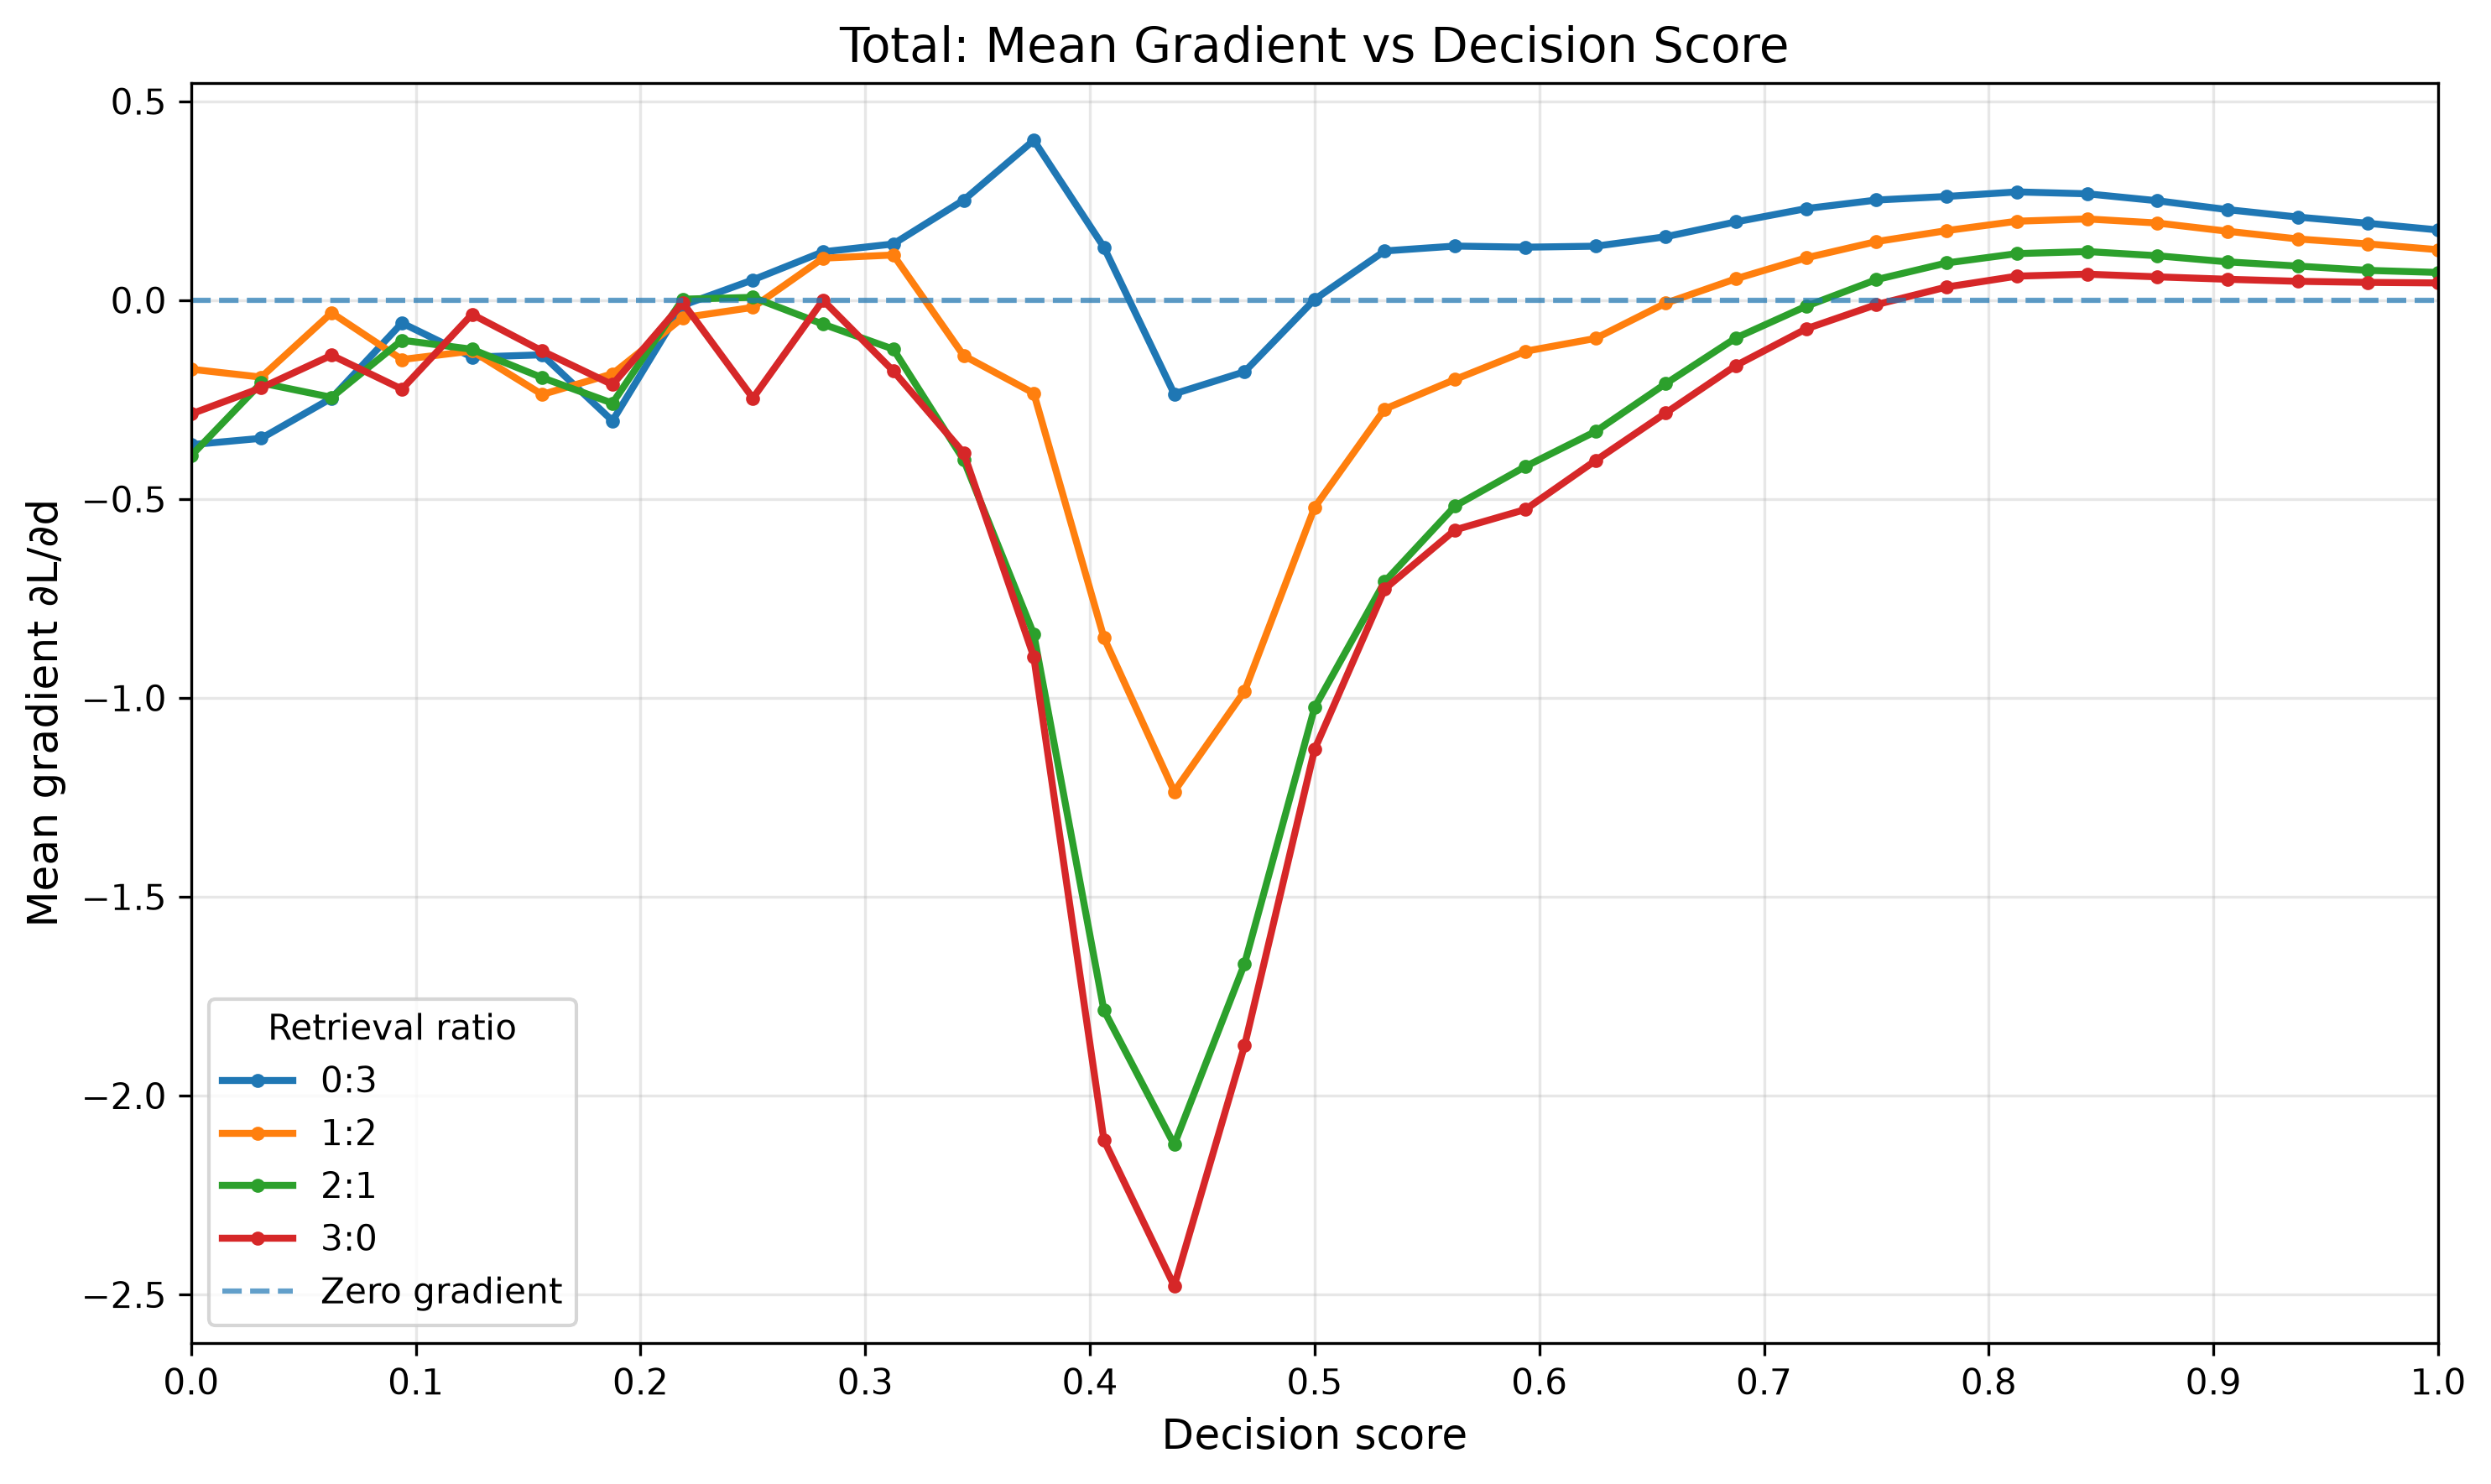
\includegraphics[width=\textwidth,height=0.78\textheight,keepaspectratio]{images/gradient_vs_decision_score_total.png}

\end{frame}